\documentclass[a4paper]{article}

\usepackage{caption}
\usepackage{listings}
\usepackage{fancyhdr}
\usepackage[top=3cm,bottom=3cm,left=3cm,right=3cm]{geometry}
\usepackage{color}
\usepackage{amsmath}
\usepackage{graphicx}
\usepackage{animate}

\definecolor{dkgreen}{rgb}{0,0.6,0}
\definecolor{gray}{rgb}{0.5,0.5,0.5}
\definecolor{mauve}{rgb}{0.58,0,0.82}

\lstset{frame=tb,
  language=Octave,
  aboveskip=3mm,
  belowskip=3mm,
  showstringspaces=false,
  columns=flexible,
  basicstyle={\small\ttfamily},
  numbers=none,
  numberstyle=\tiny\color{gray},
  keywordstyle=\color{blue},
  commentstyle=\color{dkgreen},
  stringstyle=\color{mauve},
  breaklines=true,
  breakatwhitespace=true,
  tabsize=3
}

\newcommand{\HRule}{\rule{\linewidth}{0.5mm}}
\pagestyle{fancy}
\lfoot{\small \color{gray}Tom Peerdeman - 10266186}
\cfoot{\thepage}
\rfoot{\small \color{gray}Ren\'e Aparicio Sa\'ez - 10214054}
\lhead{\small \color{gray}Autonome Mobiele Robots}

\begin{document}
\begin{titlepage}
\begin{center}
\textsc{\Large Autonome Mobiele Robots}\\[0.5cm]
\HRule \\[0,4cm]
\textsc{\huge \bfseries NXT - Localisering door middel van lijnen en blobs}
\HRule \\[8cm]
\begin{minipage}{0.4\textwidth}
\begin{flushleft}\large
\emph{Auteurs: Tom Peerdeman \& Ren\'e Aparicio Saez}\\
\end{flushleft}
\end{minipage}
\begin{minipage}{0.4\textwidth}
\begin{flushright}\large
\emph{Datum: \today\\\hspace{1cm}}\\
\end{flushright}
\end{minipage}
\end{center}
\end{titlepage}

\section{Materiaal}
Om de experimenten uit dit rapport te kunnen uitvoeren zijn de volgende materialen gebruikt:\\
- PC/Laptop met Matlab\\
- Boek: Autonomous Mobile Robots 2th Edition - Roland Siegwart et al.\\
- NXT-Robot\\
- Logitech Webcam\\
- Gloeilamp\\
- Zwarte tape

\section{Introduction}
Een autonome mobiele robot moet weten waar in de wereld hij momenteel is. Als er een kaart bekend is kan aan de hand van de omgeving die de robot momenteel detecteert bepaald worden waar in de wereld hij is. Dit kan gedaan worden aan de hand van de detectie van lijnen en blobs in zijn huidige omgeving en deze te vergelijken met de bekende blobs die opgeslagen zijn in de kaart. Gecombineerd zullen de lijnen en blobs een goede indicatie kunnen geven over de locatie van de robot.

\section{Fouten in meegeleverde code}
De meegeleverde code bevatte enkele fouten. Zo was het omzetten van het opgenomen beeld naar een zwart wit beeld 'geinverteerd' (zwart was wit en andersom). 
Tevens was het bestand imflipud.m aangepast. Het bestand imflipud.m zou een functie moeten leveren om een plaatje verticaal te spiegelen om zijn middelpunt. Het gegeven bestand bevatte echter een functie die helemaal niks deed met het plaatje.\\


\section{Maken van een dataset}
\subsection{Foto's maken}
Om experimenten uit te kunnen voeren is een dataset nodig. Deze dataset moet bestaan uit fotos die een afgeplakt parcour volledig omschrijven. Er moet hiervoor een parcour gemaakt worden met behulp van tape. Vervolgens moeten er voldoende fotos gemaakt worden zodat het gehele parcour gezien wordt. Voor de experimenten is het ook nodig dat het parcour gesloten is. Na het maken van de eerste dataset bleek er echter geen rekening gehouden te zijn met het maken van een tweede testset. Er moet opnieuw een dataset gemaakt worden op een nieuw parcour (het oude parcour is al weggegooid). Dit nieuwe parcour wordt gebruikt voor zowel de train-set als de test-set. In figuur \ref{fig:datasetmaken} is te zien hoe er te werk is gegaan bij het maken van een dataset. In figuur \ref{fig:plattegrond} is te zien hoe de uiteindelijke plattegrond van de dataset er uit is komen te zien.
\begin{figure}[h]
	\centering
	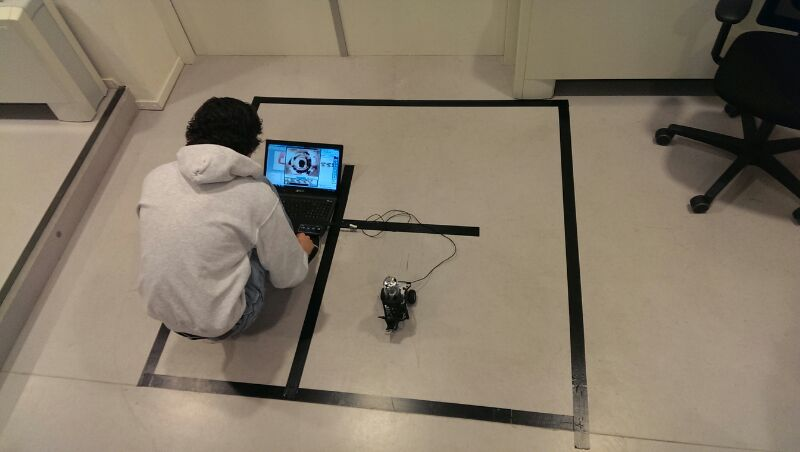
\includegraphics[width=0.7\textwidth]{dataset1.jpg}
	\caption{Het maken van een dataset (niet gebruikte dataset)}
	\label{fig:datasetmaken}
\end{figure}
\begin{figure}[h]
	\centering
	\includegraphics[width=0.8\textwidth]{opzet.png}
	\caption{Plattegrond en locaties van de gemaakte fotos}
	\label{fig:plattegrond}
\end{figure}

\subsection{Parameters}
De parameters moeten worden aangepast aan de nieuwe dataset. De camera is lichtelijk verschoven en moest verstevigd worden waardoor de positie van de lamp en het middelpunt van de camera is verplaatst ten op zichte van de vorige proeven. Het middelpunt heeft de coordinaten $x = 545$, $y = 402$. De radius blijft hetzelfde. Er zijn nog enkele uitwendige niet gebruikte sensoren van de robot afgehaald waardoor de waarden voor Rmin kan worden verlaagd. De waarde wordt verlaagd naar Rmin $= 115$. De waarde voor Rmax wordt aangepast vanwege de verplaatste locatie van de bolling ten opzichte van de camera. De waarde van Rmax wordt: Rmax $= 190$. De waarde van $\alpha$ wordt geschat door te kijken naar de manier waarop het gemeten beeld wordt 'rechtgetrokken'. De waarde veranderd naar $\alpha = 140$. Tot slot wordt de treshold voor de zwart-wit beelden aangepast. Dit wordt gedaan omdat de nieuwe opnamen geen verhoogd contrast hebben (dit was bij de vorige dataset wel het geval). De nieuwe waarde wordt  $treshold = 130$.


\section{Line fingerprints}
Met behulp van de code uit het vorige labexperiment kunnen lijnen worden gedetecteerd. Met behulp van deze code kunnen deze gevonden lijnsegmenten worden opgebouwd. Dit wordt gedaan met een meegeleverd algoritme. De gecombineerde lijnsegmenten in een foto vormen een fingerprint voor de lijnen op die locatie. In figuur \ref{fig:lijnfinger} is zo een fingerprint te zien. Door eerst te leren hoe de lijnsegmenten er uit zien. Als de robot vervolgens de testset bekijkt, worden de fingerprints die opgebouwd worden voor de test-set vergeleken met de fingerprints van de train-set. Hieruit kan de waarschijnlijkheid bepaald worden voor de huidige locatie van de robot. Dit kan worden weergegeven in een confusion matrix, zoals te zien is in figuur \ref{fig:bla}
%Toe te voegen, plaatje van goede confusion matrix%
\begin{figure}[h]
	\centering
	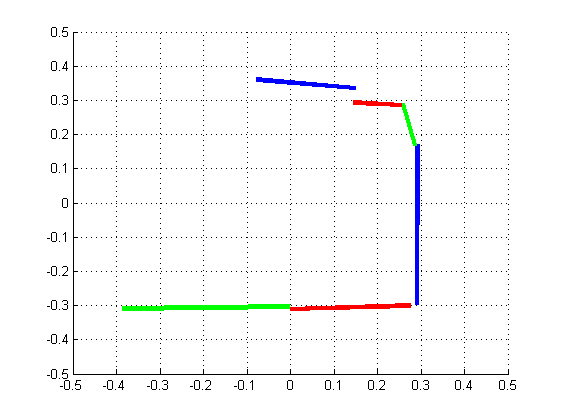
\includegraphics[width=0.8\textwidth]{fingerprint.png}
	\caption{Fingerprint voor lijnsegmenten}
	\label{fig:lijnfinger}
\end{figure}

\section{Blob fingerprints}
Met behulp van meegeleverde code wordt gezocht naar blobs. Er moet echter aangegeven worden naar welke kleurwaarden er gekeken moet worden. Aangezien er geen kleuren in het parcour zijn verwerkt moet dit worden aangepast. Door dit aan te passen zodat er alleen een onderscheidt wordt gemaakt tussen zwart en wit wordt dit overkomen. De combinatie van een de blobs in een beeld vormt een fingerprint, een voorbeeld is te zien in figuur \ref{fig:blobfinger}. Net als bij de lijnsegmenten moet worden gezocht naar een match tussen de bekende fingerprints en de huidige gemeten set blobs. Er kan weer een waarschijnlijkheid worden bepaald voor de locatie van de robot en deze kan worden weergegeven met behulp van een confusion matrix.
\begin{figure}[h]
	\centering
	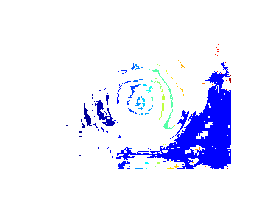
\includegraphics[width=0.8\textwidth]{fingerprintblob.png}
	\caption{Fingerprint voor blobs}
	\label{fig:blobfinger}
\end{figure}

\section{Gecombineerde fingerprints}

\section{Verbeteringen}
Momenteel worden blobs gedetecteerd die niet per se altijd in de wereld aanwezig zijn. Denk aan mensen die in de train-set als blob zijn gedetecteerd, die hoeven niet de hele tijd op dezelfde locatie te blijven staan. Daarnaast zijn de lijnen allemaal zwart. Als elke lijn een eigen kleur had gekregen had de blobdetectie waarschijnlijk beter gewerkt.

\end{document}

